\section{Implementation}

The core we design is called \texttt{aeses\_core}. It encompasses the logic
for performing encryption/decryption using Tboxes and the key scheduler, that is run
once and keeps the key material (both direct and inverse) in a proper storage.

It natively supports \textit{AES-128}, \textit{AES-192} and \textit{AES-256}.
To simplify the design, both the scheduling and encryption/decryption operations
are padded to the length of the longest version of the cipher, \textit{AES-256}.
Thus, the encryption/decryption of a block requires 15 clock cycles irrespectively of the
key size.

\subsection{Key Scheduler}

There is only one key scheduler, whose internal behaviour is also driven by the
size of the input key.

The basic building block of the key scheduling is the $g$ transformation, that
takes as input a 32-bit word.
It performs:
\begin{enumerate}
  \item \texttt{SubBytes} transformation to each byte of the 32-bit word
  \item 1-byte left rotation
  \item XOR with a round constant, $RCON$
\end{enumerate}
The bytes composing the key are arranged in columns just like the AES state depicted
in Figure \ref{fig:state}.
There are 4 columns for a 128-bit key, 6 columns for a 192-bit key and 8 columns
for a 256-bit key.
The key scheduler outputs 11/13/15 128-bit round keys according to the key length.
The way it crafts the several round keys slightly changes according to the key length.

Let $W^k_i$ be the \textit{i-th} column of the \textit{k-th} key scheduling round.
\begin{enumerate}
  \item Figure \ref{fig:aes128} shows the key scheduling round of AES-128.
$W^k_3$ goes through the $g$ transformation, then is XORed with $W^k_0$ to produce $W^{k+1}_0$.
The remaining part of the state derives from a cascade of XORs between $W^{k+1}_{i-1}$ and
$W^k_i$ with $i=1,2,3$
    \begin{figure}[h]
      \centering
      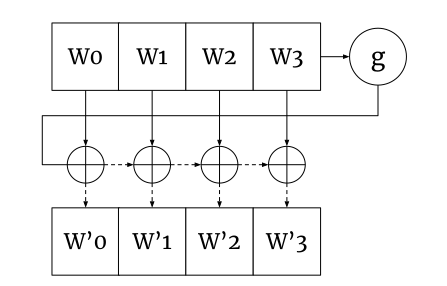
\includegraphics[width=0.4\textwidth]{figures/aes_128}
      \caption{AES-128 key scheduling round}
      \label{fig:aes128}
    \end{figure}
  \item Figure \ref{fig:aes192} shows the key scheduling round of AES-192.
It is identical to the previous one, but this time the chain of XORs is longer in order to
produce a 192-bit key scheduling state
    \begin{figure}[h]
      \centering
      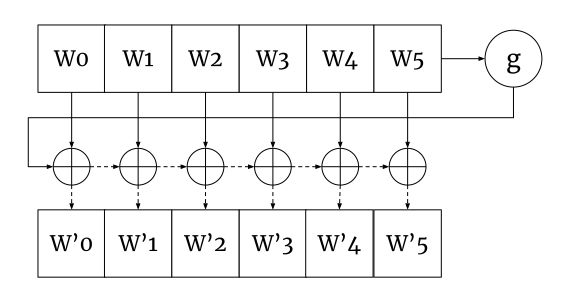
\includegraphics[width=0.5\textwidth]{figures/aes_192}
      \caption{AES-192 key scheduling round}
      \label{fig:aes192}
    \end{figure}
  \item Finally, Figure \ref{fig:aes256} shows the key scheduling round of AES-256.
While the scheduler  updates the first 128 bits of the state in the same exact way as AES-128,
there is an additional \texttt{SubBytes} transformation involving $W^{k+1}_3$ before going on with
the chain of XORs.
    \begin{figure}[h]
      \centering
      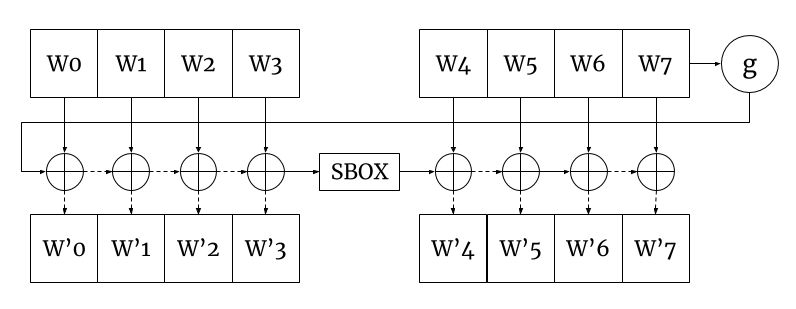
\includegraphics[width=0.6\textwidth]{figures/aes_256}
      \caption{AES-256 key scheduling round}
      \label{fig:aes256}
\end{figure}
\end{enumerate}

In order to unify the datapath of the key scheduler for the three different key sizes, we keep
a 256-bit state inside the key scheduler. It is split into 8 32-bit registers, named
\texttt{key\_word\_register[0:7]}.
When a new key schedule is requested, we first initialize them with the incoming 256-bit
key -- padded if necessary.

The key scheduler is capable of producing a 128-bit round key per clock cycle once it starts
its operation.
If the key size is 128-bit, we update only the lower \texttt{key\_word\_register[0:3]}, while
the \textit{write enable} of the other ones is disabled.

In a 256-bit schedule, we distinguish two phases: in the \textit{even phases} we update,
only the lower
\texttt{key\_word\_register[0:3]}, while in the \textit{odd phases}, only the upper
\texttt{key\_word\_register[4:7]}.

In both these cases, when we produce the new internal state to be written at the end of the
current clock cycle, we also output the old one already stored inside the registers.

Finally, in a 192-bit schedule, there are three phases.
During the \textit{first phase}, \texttt{key\_word\_register[0:5]} are updated. In the meanwhile,
the old \texttt{key\_word\_register[0:3]} are output. The old \texttt{key\_word\_register[4:5]}
are buffered in two additional registers, named \texttt{alternate\_buffer[0:1]}. They would be otherwise
overwritten
during the \textit{second phase}, when again \texttt{key\_word\_register[0:5]} are updated. The
\texttt{alternate\_buffer[0:1]} and the \texttt{key\_word\_register[0:1]} produced in the first
phase are output.
Finally, in the \textit{third phase}, no state register is written and the last
\texttt{key\_word\_register[2:5]} are output.

The correct output for each clock cycle is selected according to the phase number and the
key size.

\subsection{Encryption/Decryption Datapath}

The structure of the encryption/decryption datapath is significantly easier.
In fact, once we store the direct and inverse key schedule, the only thing
that differentiates each key size is the number of rounds, which is 10/12/14 respectively
for AES-128/192/256. This is achieved by initializing the \texttt{round\_count} to 4/2/0
respectively, and ending the computation when it hits the value 13.

When \texttt{round\_count} is equal to 13, no \texttt{MixColumns} or \texttt{InvMixColums}
needs to be performed, thus the output consists of the outcome of the Sboxes rather than
Tboxes, for both encryption and decryption.

Finally, thanks to the optimizations introduced in Section \ref{sec:inv_tbox}, we just need to
either use direct or inverse Tboxes and key schedule to perform an encryption or decryption respectively.
The inputs to this module, \texttt{round\_key} and \texttt{inv\_round\_key} are supposed to be the
correct ones since the moment the signal \texttt{start\_operation} is asserted.
The wrapping module has to ensure this invariant.

\subsection{Host Controller}

The \texttt{host\_ctrl} module connects the provided \texttt{aeses\_core} to a \textit{UART}
interface.
The host controller is in charge of issuing commands to the AES core and collecting the results
of encryptions and decryptions.

The original version only supported either encryption or decryption of AES-128.
In order to extend the functionality of our implementation, the user now needs to send a so called
\texttt{AESES\_CONTROL\_BYTE}, that instructs the \texttt{aeses\_core} to: sit idle, create a new
key schedule, encrypt or decrypt a 128-bit data block.

The format of the \texttt{AESES\_CONTROL\_BYTE} is defined in Table \ref{tab:aeses_byte}.

\begin{table}[h]
  \caption{\texttt{AESES\_CONTROL\_BYTE} encoding}
  \label{tab:aeses_byte}
  \begin{tabularx}{\textwidth}{| c | X | X | X |}
    \hline
    Bits & Function & Values & Behaviour \\
    \hline
    \hline
    7 & RESET\newline New key schedule & 0 -- disabled\newline1 -- enabled & Start a new key schedule and wait for 32 bytes from UART \\
    \hline
    6-5 & Key size & 00 -- AES-128\newline01 -- AES-192\newline1X -- AES-256 & Only taken into account if RESET=1\\
    \hline
    4 & EN\newline Enable AES & 0 -- idle \newline1 -- enable core & Valid only if RESET=0. It waits for 16 data bytes from UART\\
    \hline
    3 & ENC\_DEC & 1 -- encryption\newline0 -- decryption & Valid only if EN=1 and RESET=0 \\
    \hline
    2-0 & Unused & XXX & \texttt{AESES\_CONTROL\_BYTE} padding \\
    \hline
  \end{tabularx}
\end{table}

\subsection{Main Components Interface}

Here we present the input/output signals of the designed modules.
All of them receive a \texttt{clk} and \texttt{rst} signal from the top level module,
called \texttt{fpga\_top} in the project sources.
The reset is \textit{synchronous} and \textit{active high} throughout \texttt{aeses\_core}.

\subsubsection{\texttt{aeses\_core}}

The AES top-level module is shown in Figure \ref{fig:aeses_core}.

\begin{figure}[h]
  \centering
  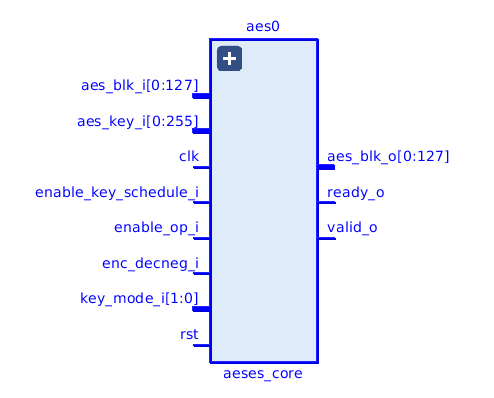
\includegraphics[width=0.5\textwidth]{figures/aeses_core}
	  \caption{Interface of the \texttt{aeses\_core}}
  \label{fig:aeses_core}
\end{figure}

It has three possible \textbf{internal states}:
\begin{enumerate}
	\item \texttt{READY}: the core is ready to do something, be it a new key-schedule
or and encryption/decryption;
	\item \texttt{SCHEDULING}: the core is calculating a key-schedule;
	\item \texttt{OPERATION}: the core is encrypting/decrypting a block of data.
\end{enumerate}

A brief documentation of the \textbf{input signals}:
\begin{itemize}
	\item \texttt{aes\_blk\_i}: input plaintext/ciphertext
	\item \texttt{aes\_key\_i}: input key for AES
	\item \texttt{enable\_key\_schedule\_i}: when the core is \texttt{READY} and the signal
is asserted for 1 clock cycle, start a new key scheduling operation with \texttt{aes\_key\_i}
	\item \texttt{enable\_op\_i}: when the core is \texttt{READY} and the signal is asserted
for 1 clock cycle, start a new encryption/decryption operation. If both \texttt{enable\_op\_i}
and \texttt{enable\_key\_schedule\_i} are asserted, the latter has the precedence.
	\item \texttt{enc\_decneg\_i}: if 1, encrypt the data block, otherwise decrypt. It needs to
be correctly set only when \texttt{enable\_op\_i} is asserted, it is otherwise ignored.
	\item \texttt{key\_mode\_i}: specifies the length of the key, according to the encoding
established in Table \ref{tab:aeses_byte}. It needs to
be correctly set only when \texttt{enable\_key\_sched\_i} is asserted, it is otherwise ignored.
\end{itemize}

A brief documentation of the \textbf{output signals}:
\begin{itemize}
	\item \texttt{ready\_o}: asserted when the core is in the \texttt{READY} state
	\item \texttt{aes\_blk\_o}: this is the output of an AES encryption/decryption
	\item \texttt{valid\_o}: asserted then \texttt{aes\_blk\_o} is valid
\end{itemize}

\subsubsection{\texttt{double\_scheduler}}

The module performing the key scheduling operation is shown in Figure \ref{fig:key_scheduler}

\begin{figure}[h]
  \centering
  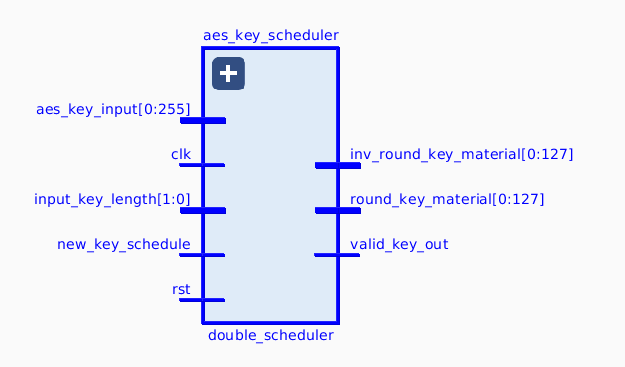
\includegraphics[width=0.5\textwidth]{figures/key_scheduler}
	  \caption{Interface of the \texttt{key\_scheduler}}
  \label{fig:key_scheduler}
\end{figure}

A brief documentation of \textbf{input signals}:
\begin{itemize}
	\item \texttt{aes\_key\_input}: the key being scheduled
	\item \texttt{input\_key\_lenght}: specifies the correct key length
	\item \texttt{new\_key\_schedule}: starts a new key scheduling operation
\end{itemize}

A brief documentation of \textbf{output signals}:
\begin{itemize}
	\item \texttt{inv\_round\_key\_material}: the round key for the inverse key schedule (decryption)
	\item \texttt{round\_key\_material}: the direct round key for encryption
	\item \texttt{valid\_key\_out}: set when the previous outputs are valid
\end{itemize}

The key-scheduler outputs round keys at the rate of 1 round key/clock cycle.
The modules storing this information need to be fast enough to catch them, otherwise
they are lost.

\subsubsection{\texttt{shift\_register}}

It holds the round keys for encryption. It is shown in Figure \ref{fig:key_store}.

\begin{figure}[h]
  \centering
  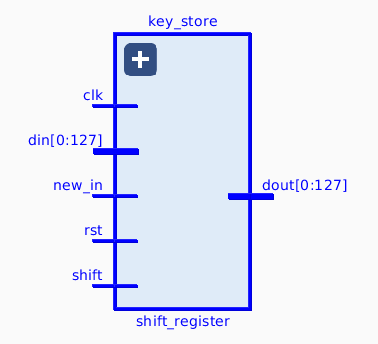
\includegraphics[width=0.5\textwidth]{figures/key_store}
	  \caption{Interface of the \texttt{shift\_register}}
  \label{fig:key_store}
\end{figure}

This module has a \textit{read end} and a \textit{write end} and does not allow
random access to its internal storage.

During a write operation, the internal data-words are shifted forward in the next
slot. If the size of the storage is exceeded, older data is lost.

During a read operation, the data from the read-end is output and the register is
shifted forward. However, the output data is written back to the queue, thus implementing
a circular data structure.

A brief documentation of \textbf{input signals}:
\begin{itemize}
	\item \texttt{din}: input data
	\item \texttt{new\_in}: writes a new chunk of data at the write-end
	\item \texttt{shift}: if set, move the shift register forward
\end{itemize}

A brief documentation of \textbf{output signals}:
\begin{itemize}
	\item \texttt{dout}: data stored at the read end
\end{itemize}

The module \texttt{circular\_lifo} behaves similarly, but it actually implements a
"cirular" stack for storing the inverse key schedule.

\subsubsection{\texttt{aes\_cipher}}

The module performing encyrption/decryption of AES blocks is shown in Figure \ref{fig:aes_cipher}.

\begin{figure}[h]
  \centering
  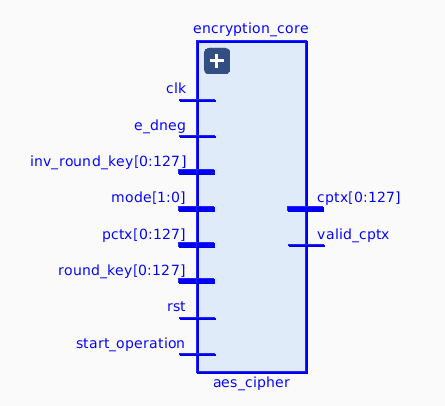
\includegraphics[width=0.5\textwidth]{figures/aes_cipher}
	  \caption{Interface of the \texttt{aes\_cipher}}
  \label{fig:aes_cipher}
\end{figure}

A brief documentation of \textbf{input signals}:
\begin{itemize}
	\item \texttt{e\_dneg}: needs to be correctly set during the whole encryption/decryption process.
If 1, encrypt, otherwise decrypt.
	\item \texttt{start\_operation}: when asserted for one clock cycle, start a new operation.
	\item \texttt{mode}: key schedule length. Needs to be correctly set only when \texttt{start\_operation}
is asserted.
	\item \texttt{pctx}: AES input block
	\item \texttt{round\_key} and \texttt{inv\_round\_key}: the correct 128-bit words for the
key addition phase.

\end{itemize}

A brief documentation of \textbf{output signals}:
\begin{itemize}
	\item \texttt{cptx}: output AES block
	\item \texttt{valid\_cptx}: if set for 1 clock cycle, the output is valid
\end{itemize}

Since the very moment \texttt{start\_operation} is asserted, the module requires
the correct round keys to materialize at its input ports. A round key is consumed
every clock cycle, and if the top level module doesn't keep up with this rate, the
results will be wrong.

\subsection{\texttt{\textbf{aeses\_lite}}}

The lightweight implementation of \textit{AES-256} for \textit{ECB encryption} is based
on a stripped down version of the full \texttt{aeses\_core}. It has been designed
to achieve the maximum possible working frequency and reduce the footprint.
